\documentclass{article}

\usepackage{a4wide}
\usepackage[utf8]{inputenc}
\usepackage[T1]{fontenc}
\usepackage[french]{babel}
\usepackage[babel=true]{csquotes} % guillemets français
\usepackage{graphicx}
\graphicspath{{Images/}}
\usepackage{color}
\usepackage{hyperref}
\hypersetup{colorlinks,linkcolor=,urlcolor=blue}
\usepackage{amsmath}
\usepackage{amssymb}


\title{Rapport jeu de dame, Android, IOS}
\author{Billy Ronico, Said Ismael, L3 informatique}
\date{\today}

\begin{document}

\maketitle % pour écrire le titre


\section{Introduction}
\label{section:intro} % pour faire référence à la section ailleurs (\ref{...} voir plus bas)

Dans le cadre de la licence informatique, plus précisement dans le cours de developpement 
mobile, nous avons choisi de réaliser \textbf{un jeu de dame} sur Android et IOS.

\section{\textit{Regle du jeu de dame}~\cite{regleJeuDame}} 

\begin{itemize}
  \item Le jeu se joue à 2 joueurs sur un plateau de taille n * n.
  \item Les joueurs jouent chacun à leur tour. Les blancs commencent toujours.
  \item Le but du jeu est de capturer tous les pions adverses. 
  \item Si un joueur ne peut plus bouger, même s'il lui reste des pions, il perd la partie. 
  \item Chaque pion peut se déplacer d'une case vers l'avant en diagonale. 
  \item Un pion arrivant sur la dernière rangée et s'y arrêtant est promu en « dame ».
  \item La dame se déplace sur une même diagonale d'autant de cases qu'elle le désire, en avant et en arrière.
  \item Un pion peut en prendre un autre en sautant par dessus le pion adverse
   pour se rendre sur la case vide située derrière celui-ci. Le pion sauté est retiré du jeu.
  \item La prise est obligatoire.
  \item Lorsque plusieurs prises sont possibles, 
  il faut toujours prendre du côté du plus grand nombre de pièces.
  \item La dame doit prendre tout pion situé sur sa diagonale 
  (s'il y a une case libre derrière) et doit changer de direction à chaque 
  fois qu'une  nouvelle prise est possible. 
\end{itemize}

\section{Description générale de l'application}

Voici une capture du menu principal et d'une partie du jeu

\begin{center}
  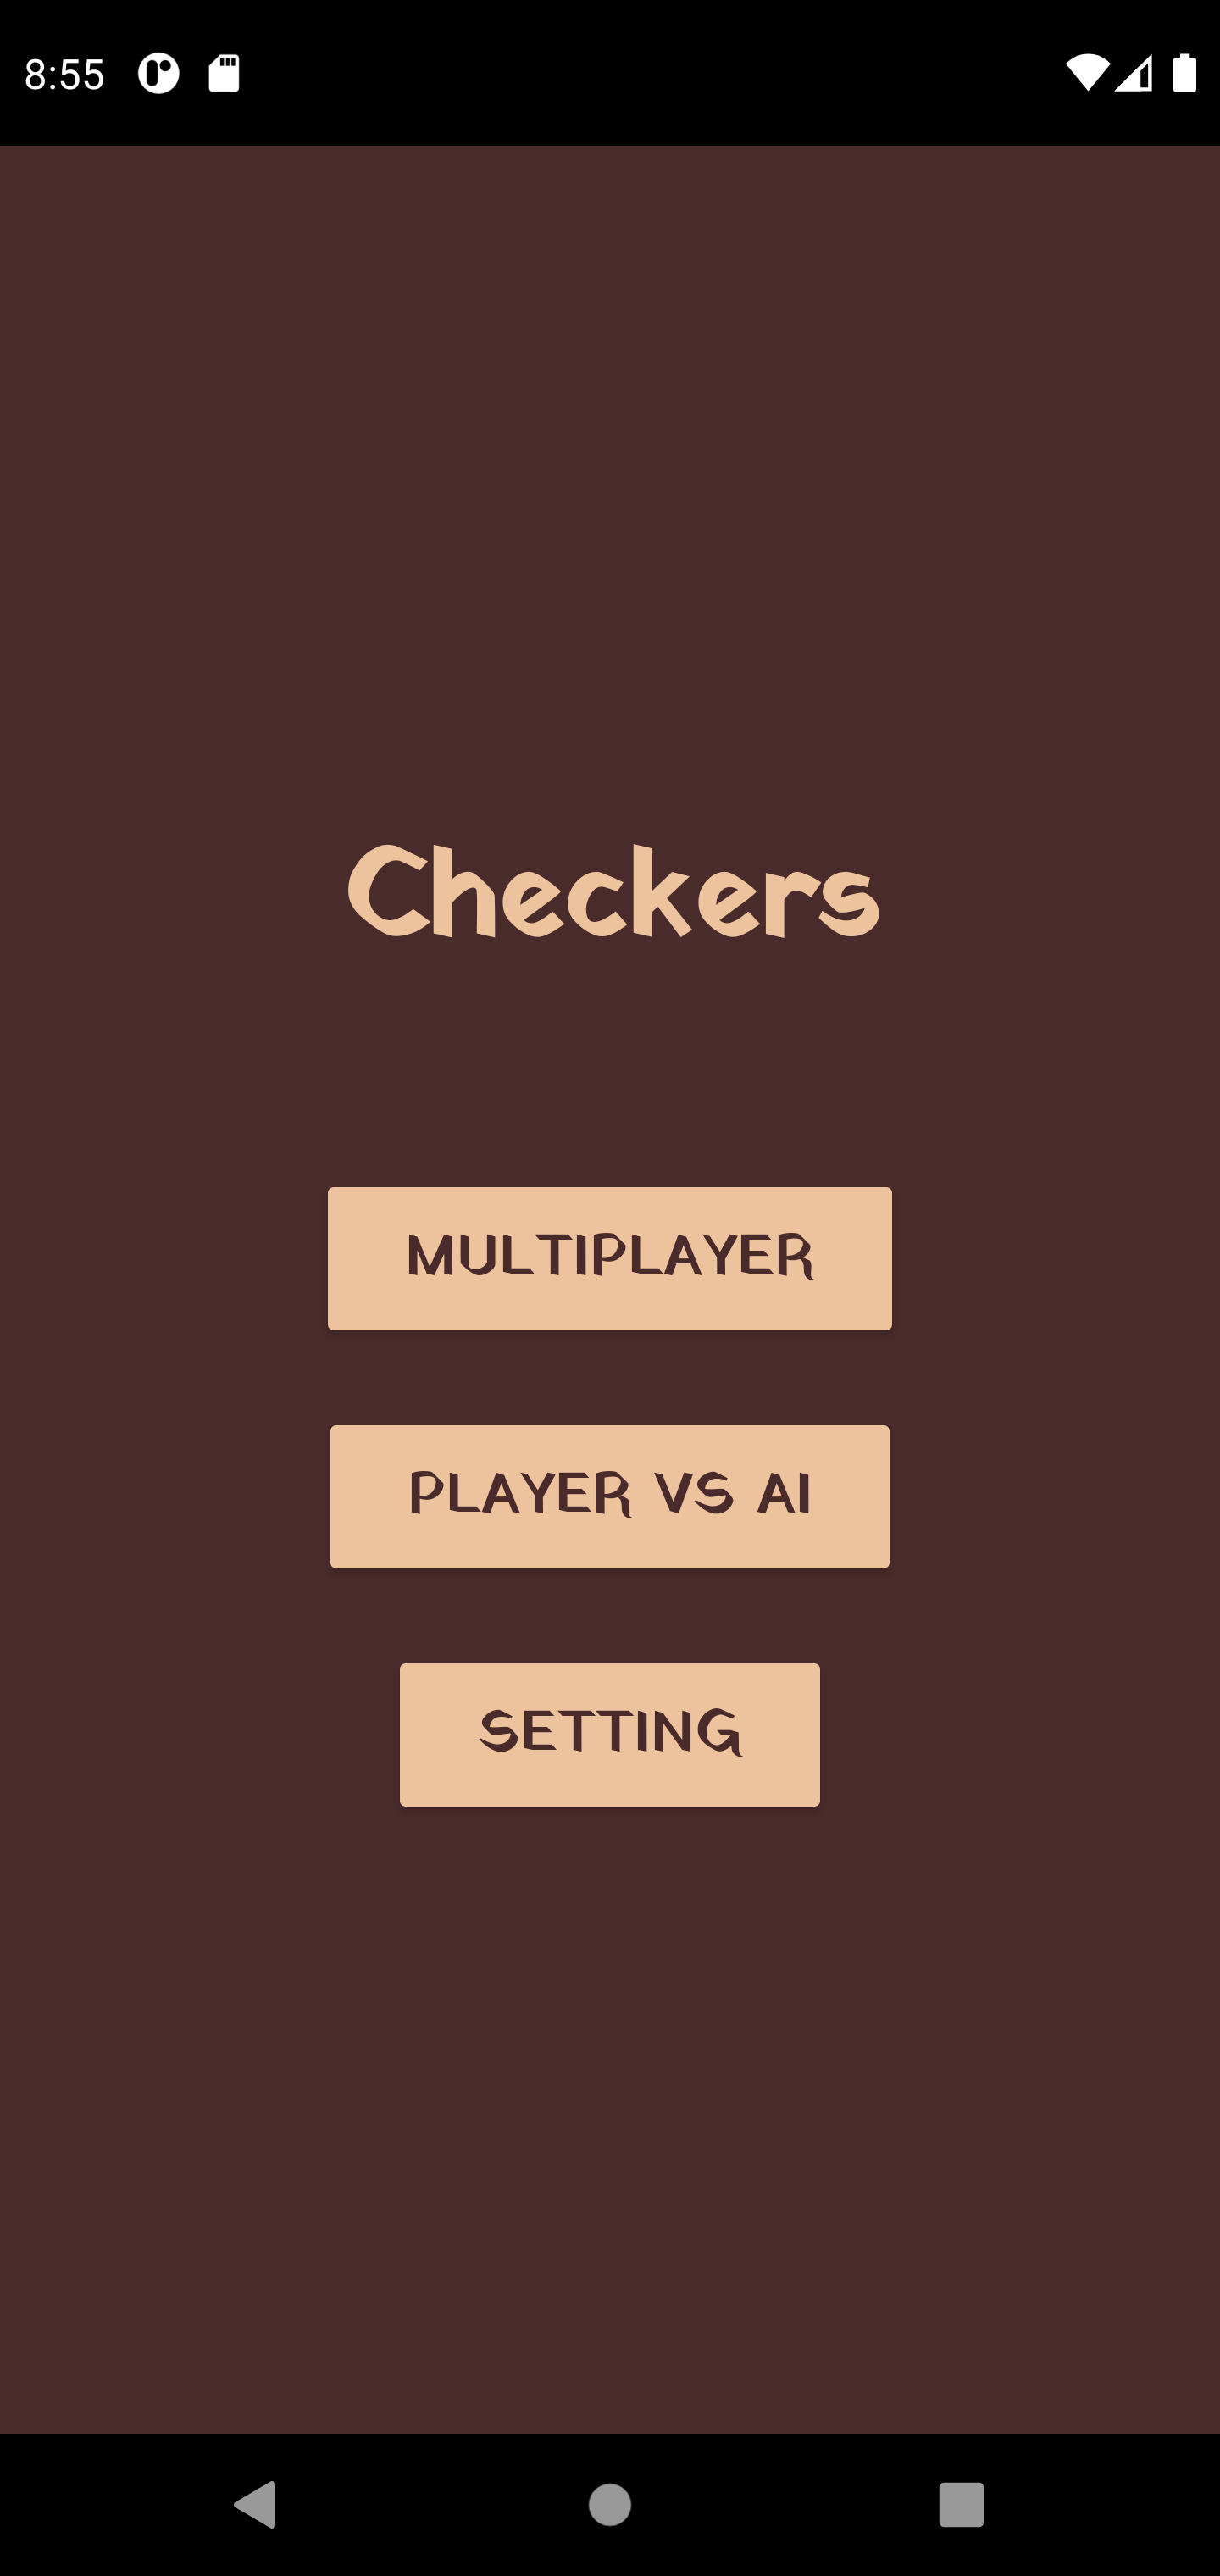
\includegraphics[scale=0.1]{menu_principal.png}
  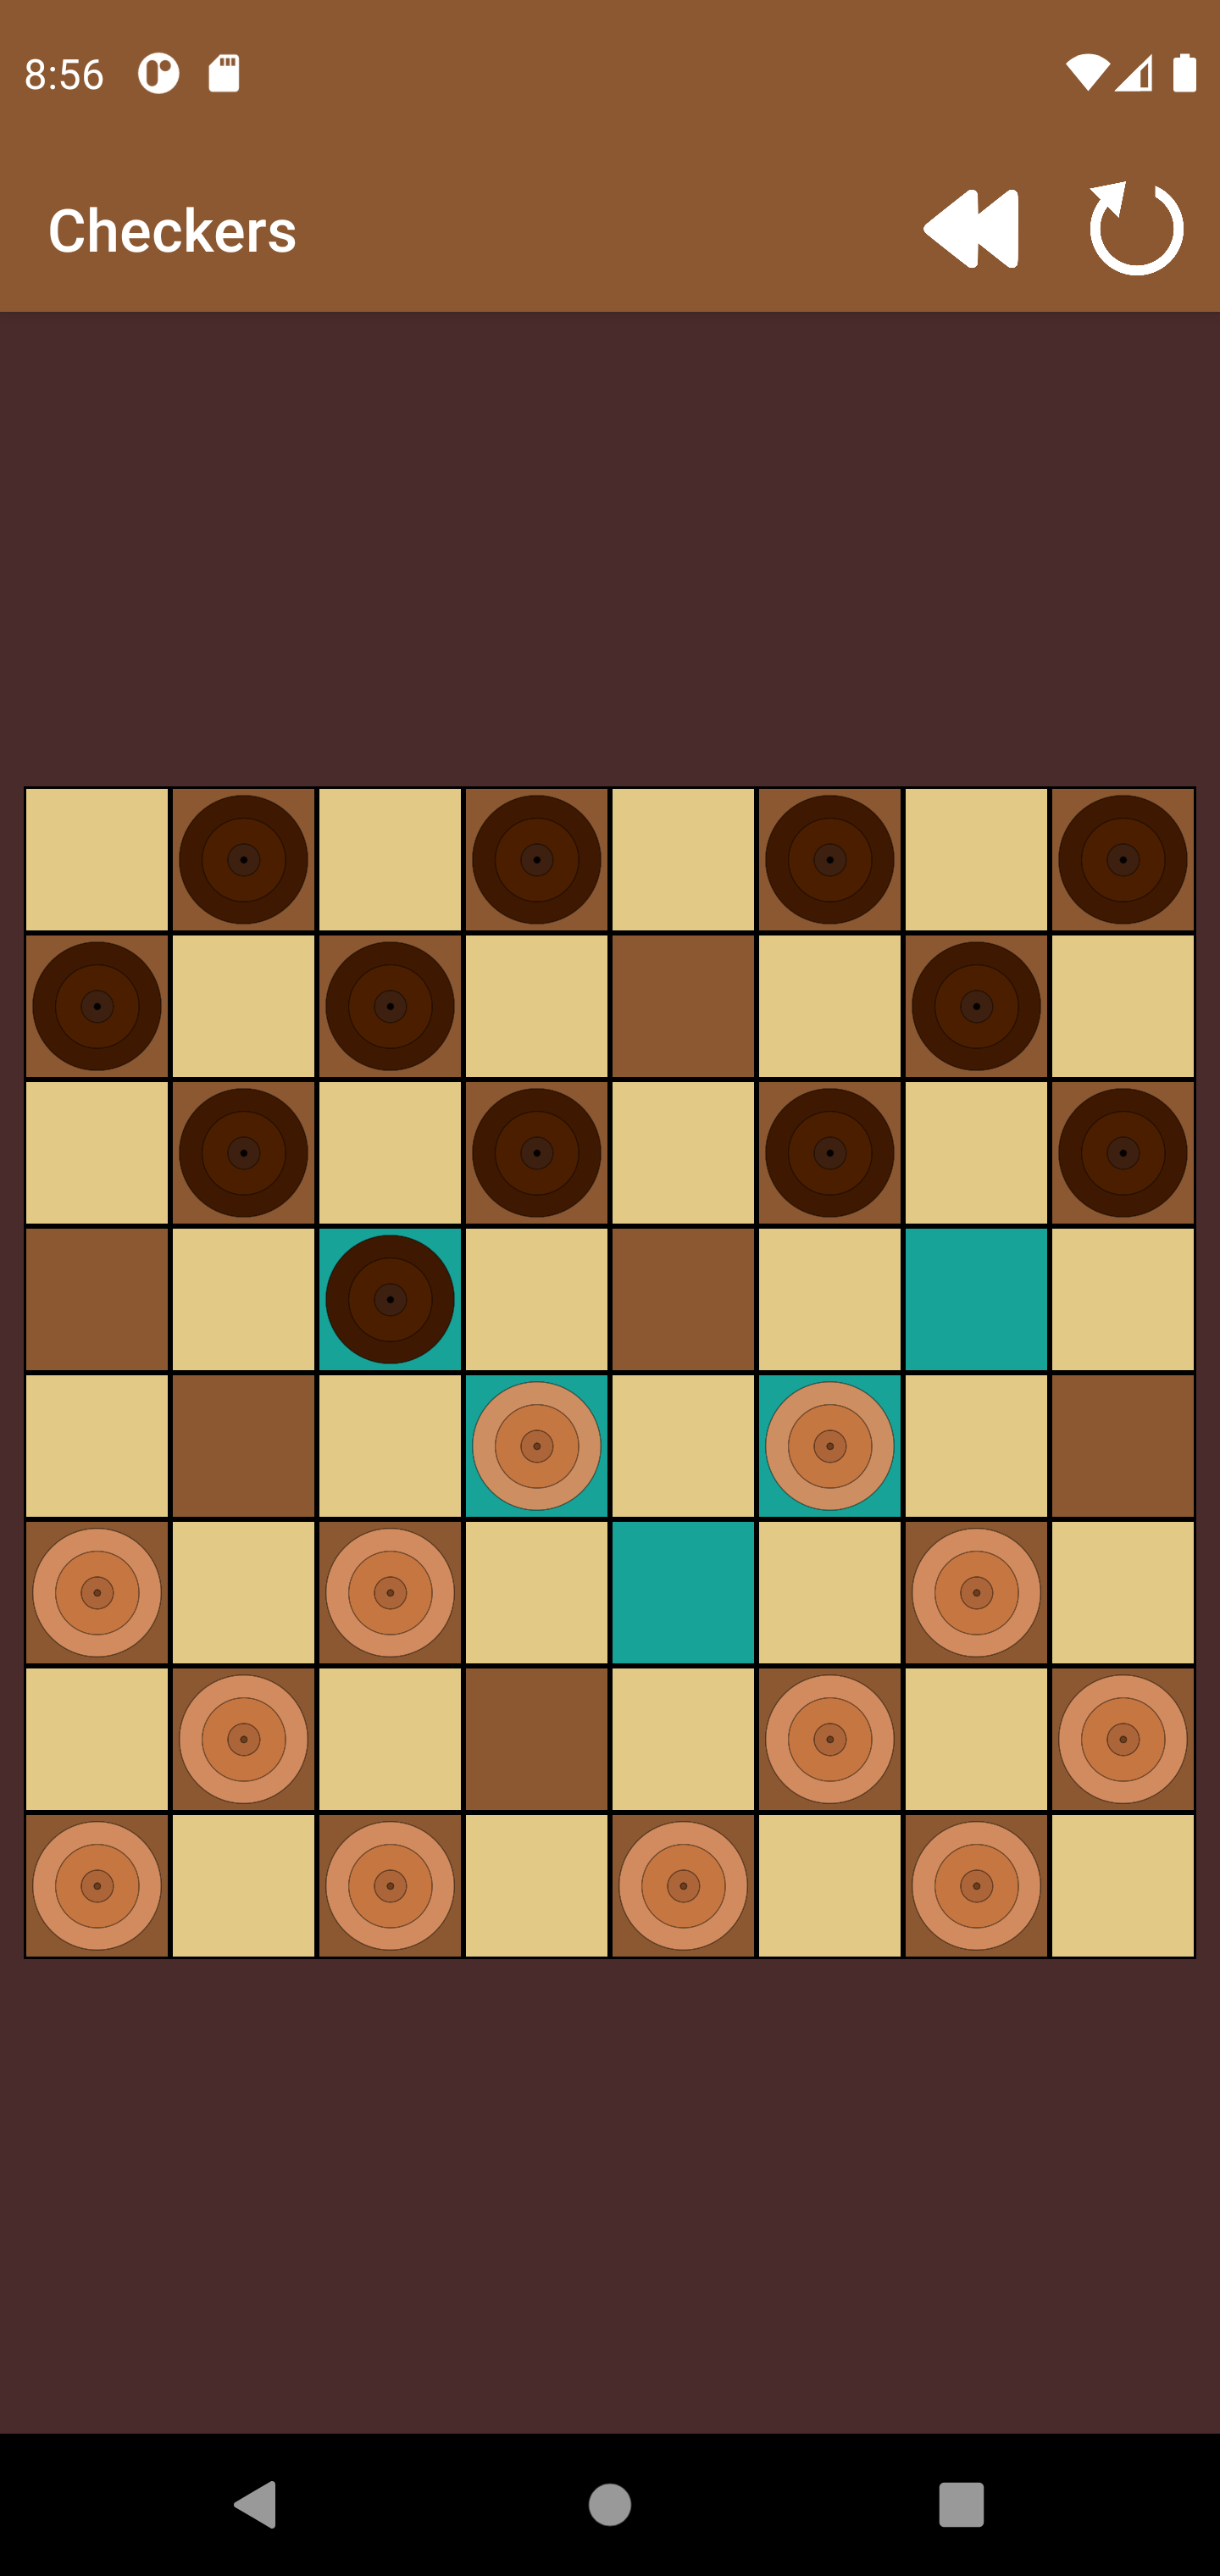
\includegraphics[scale=0.1]{partie_1.png}
\end{center}

\textbf{Fonctionnalités proposé par le jeu:}

\begin{enumerate}
\item Un mode multijoueur:

Ce mode consiste à faire affronté 2 joueurs sur un même plateau de jeu.

Les joueurs joue tour par tour sur les 2 cotés du téléphone. 
De ce fait, pour des raisons d'IHM, on a décidé d'éxclure le mode \textit{paysage} du jeu

\item Un mode joueur contre une \textbf{Inteligence Artificielle}

Ce mode consiste à faire affronté un joueur contre un IA.
L'IA a été implémenté en utilisant l'algorithme \textit{minimax}~\cite{miniMax}

\item Paramètres
Permet de personnaliser la couleur des cases, le taille du damier (6*6, 8*8, 10*10) 
et la difficulté de l'IA (Facile, Moyen, Difficile)

\begin{center}
  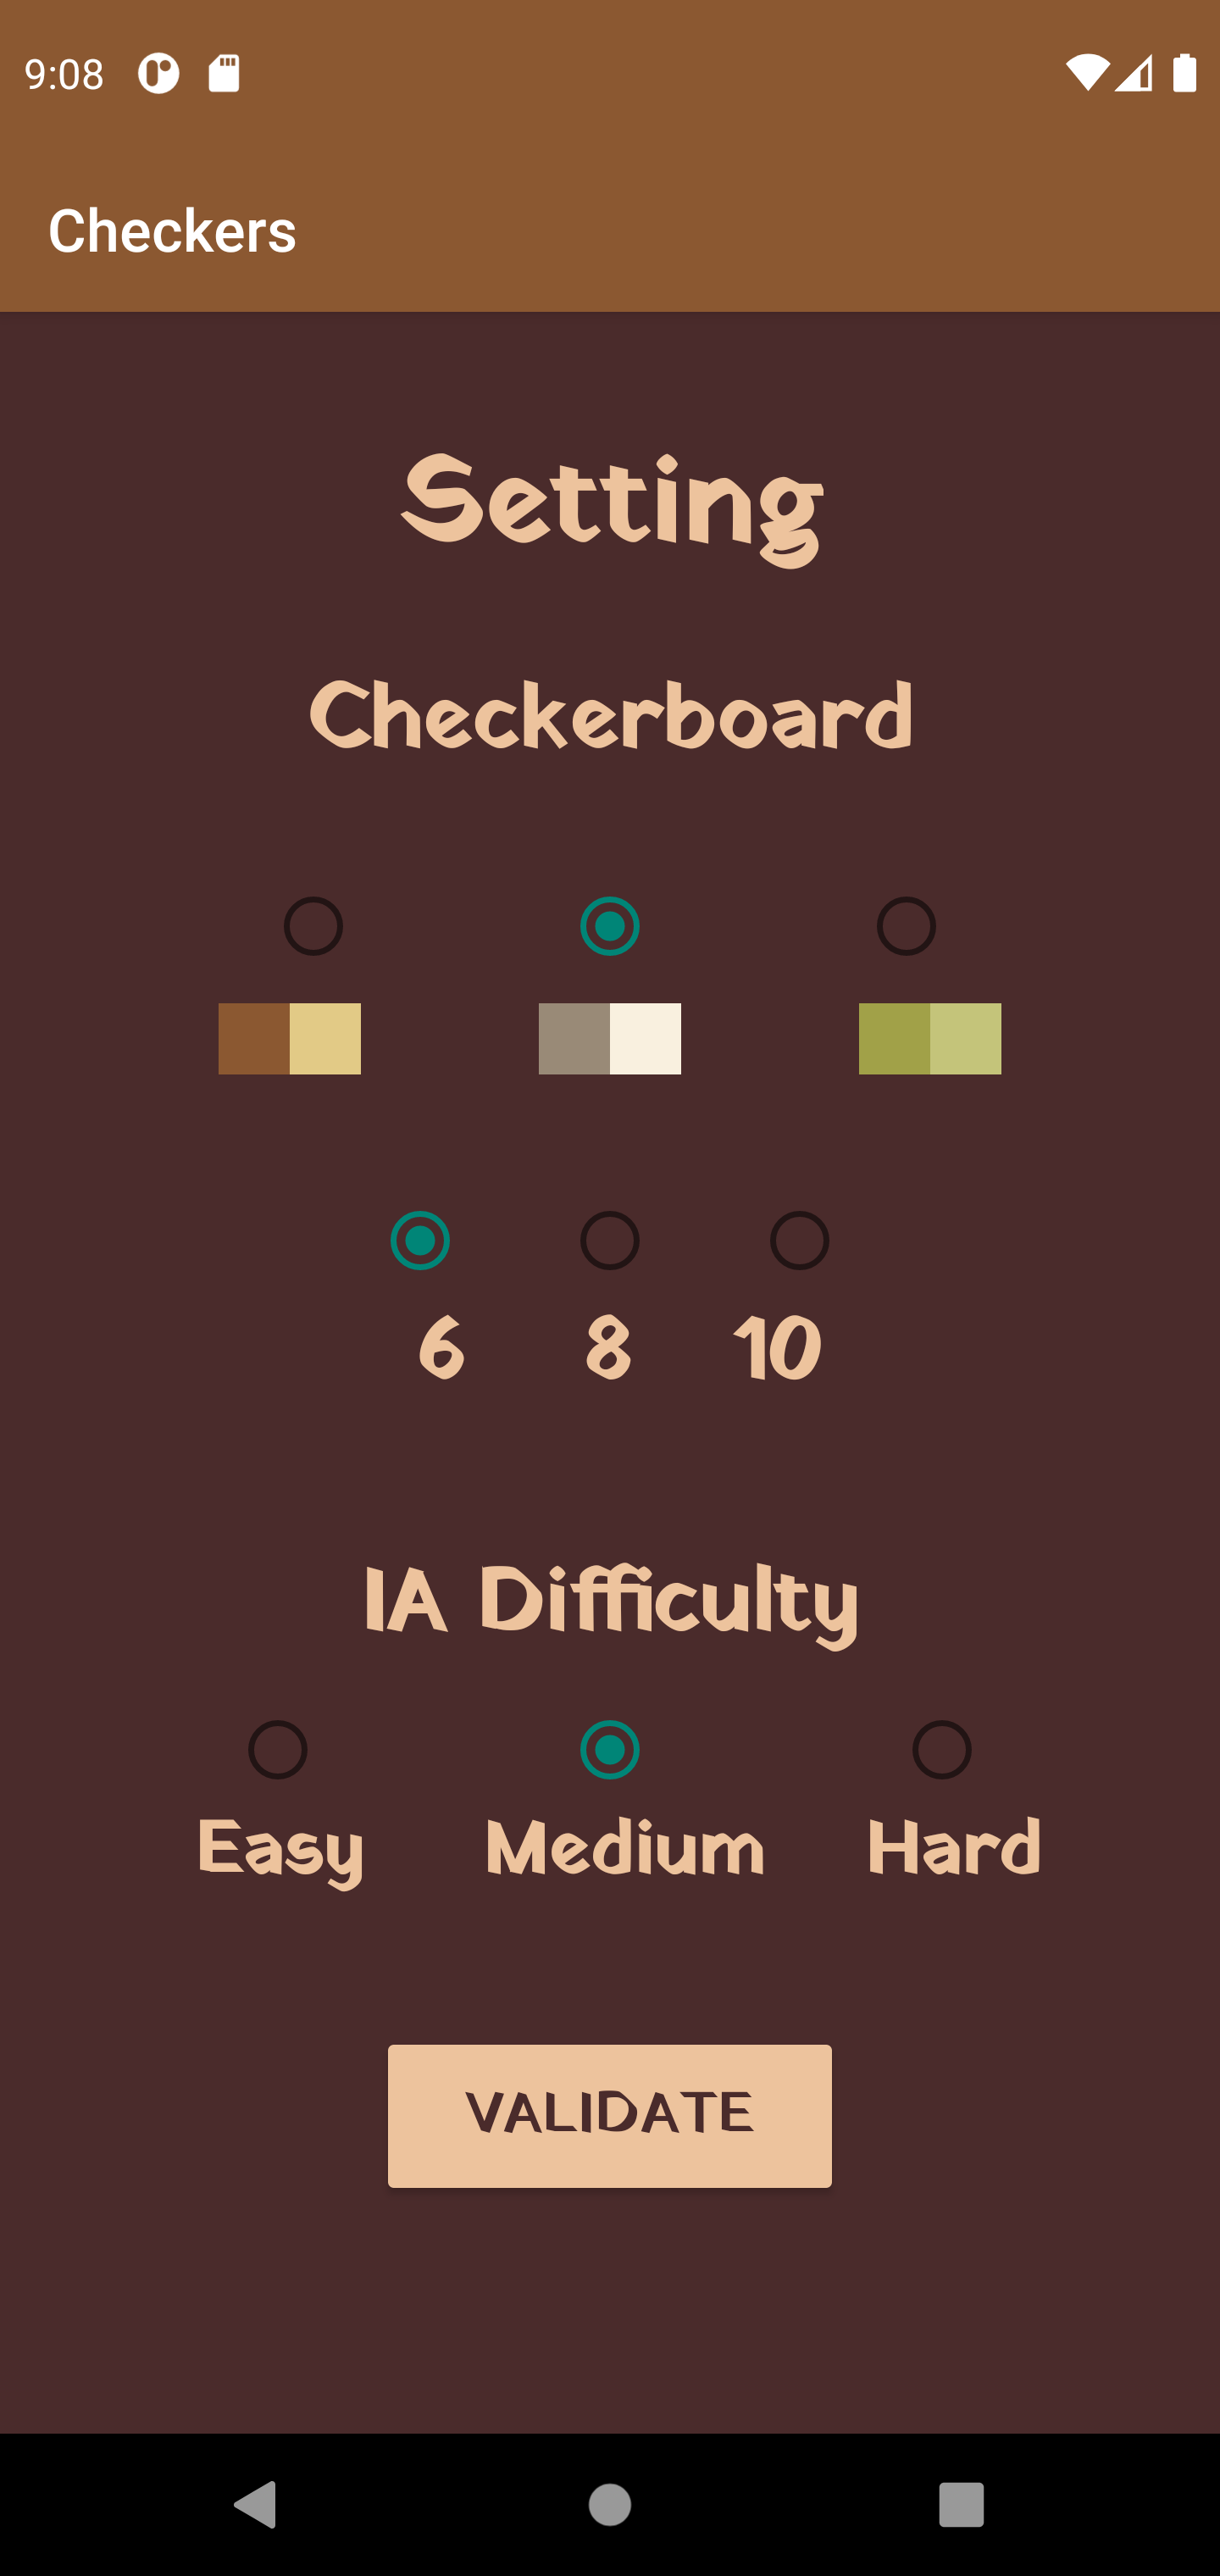
\includegraphics[scale=0.1]{setting_en.png}
  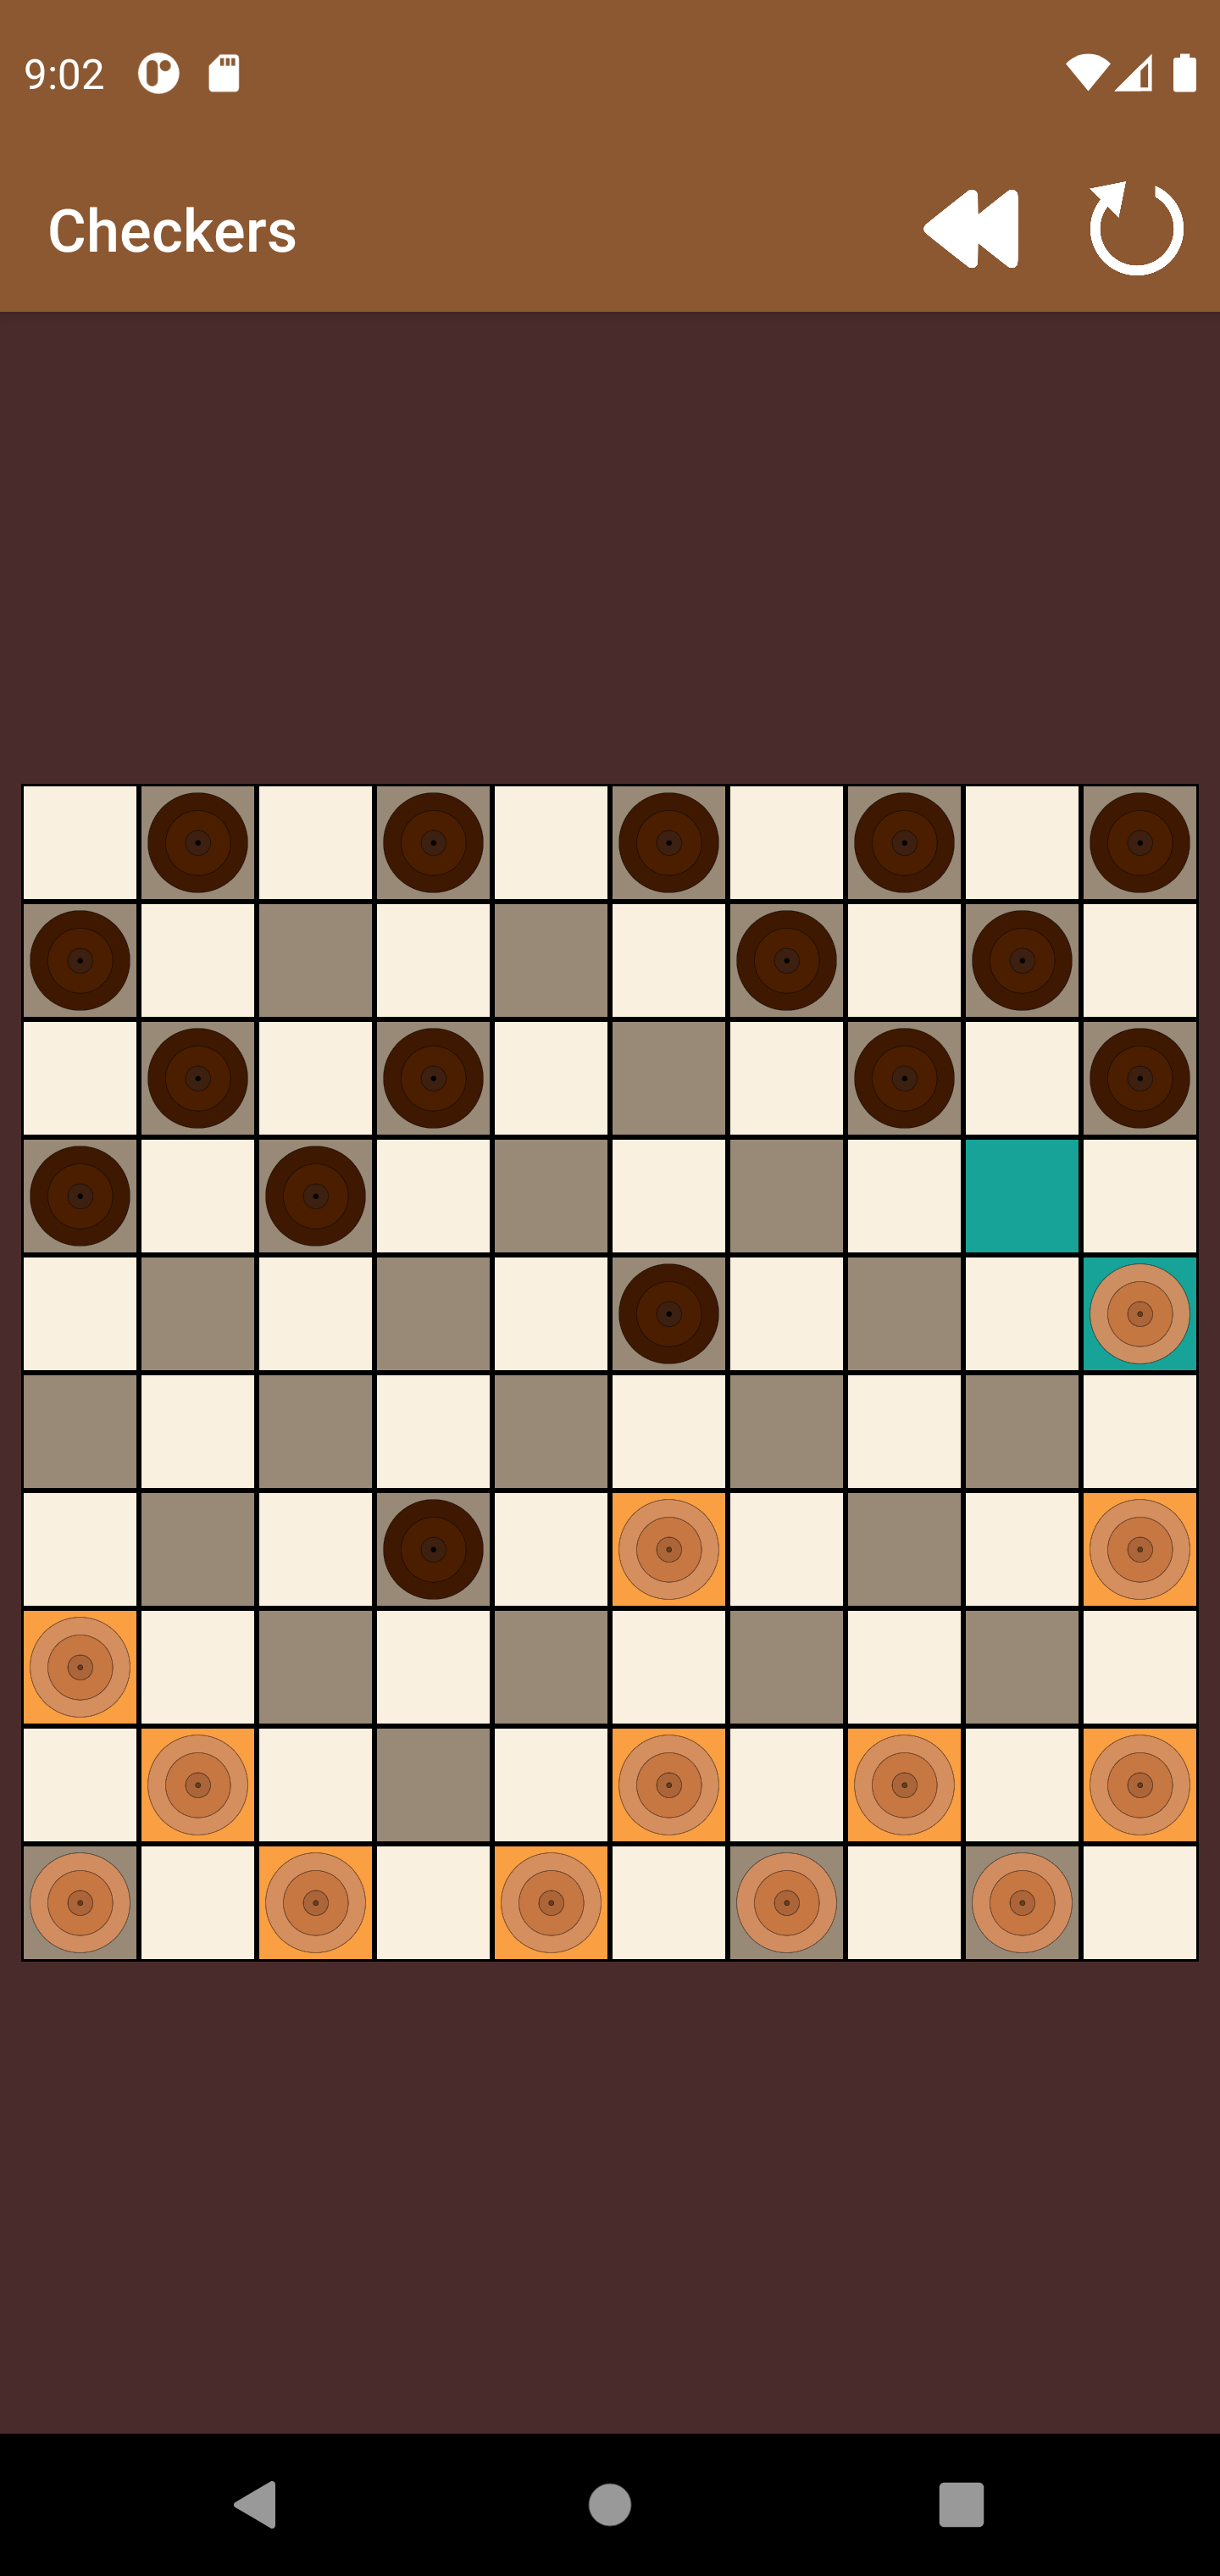
\includegraphics[scale=0.1]{partie_2.png}
\end{center}

\item Option retour en arrière (<<)
Le bouton gauche de l'OptionMenu qui permet de revenir en arrière sur 
la partie en cours (disponible sur les 2 modes de jeu cité ci-dessus)

\item Option restart Game
Le bouton droit de l'OptionMen qui permet de restart la partie en cours

\item Application bilingue et responsive

L'application est disponible en français (par défaut) et en anglais.

De plus, l'applcation est résponsive, et s'adapte sur tout taille d'écran.

\begin{center}
  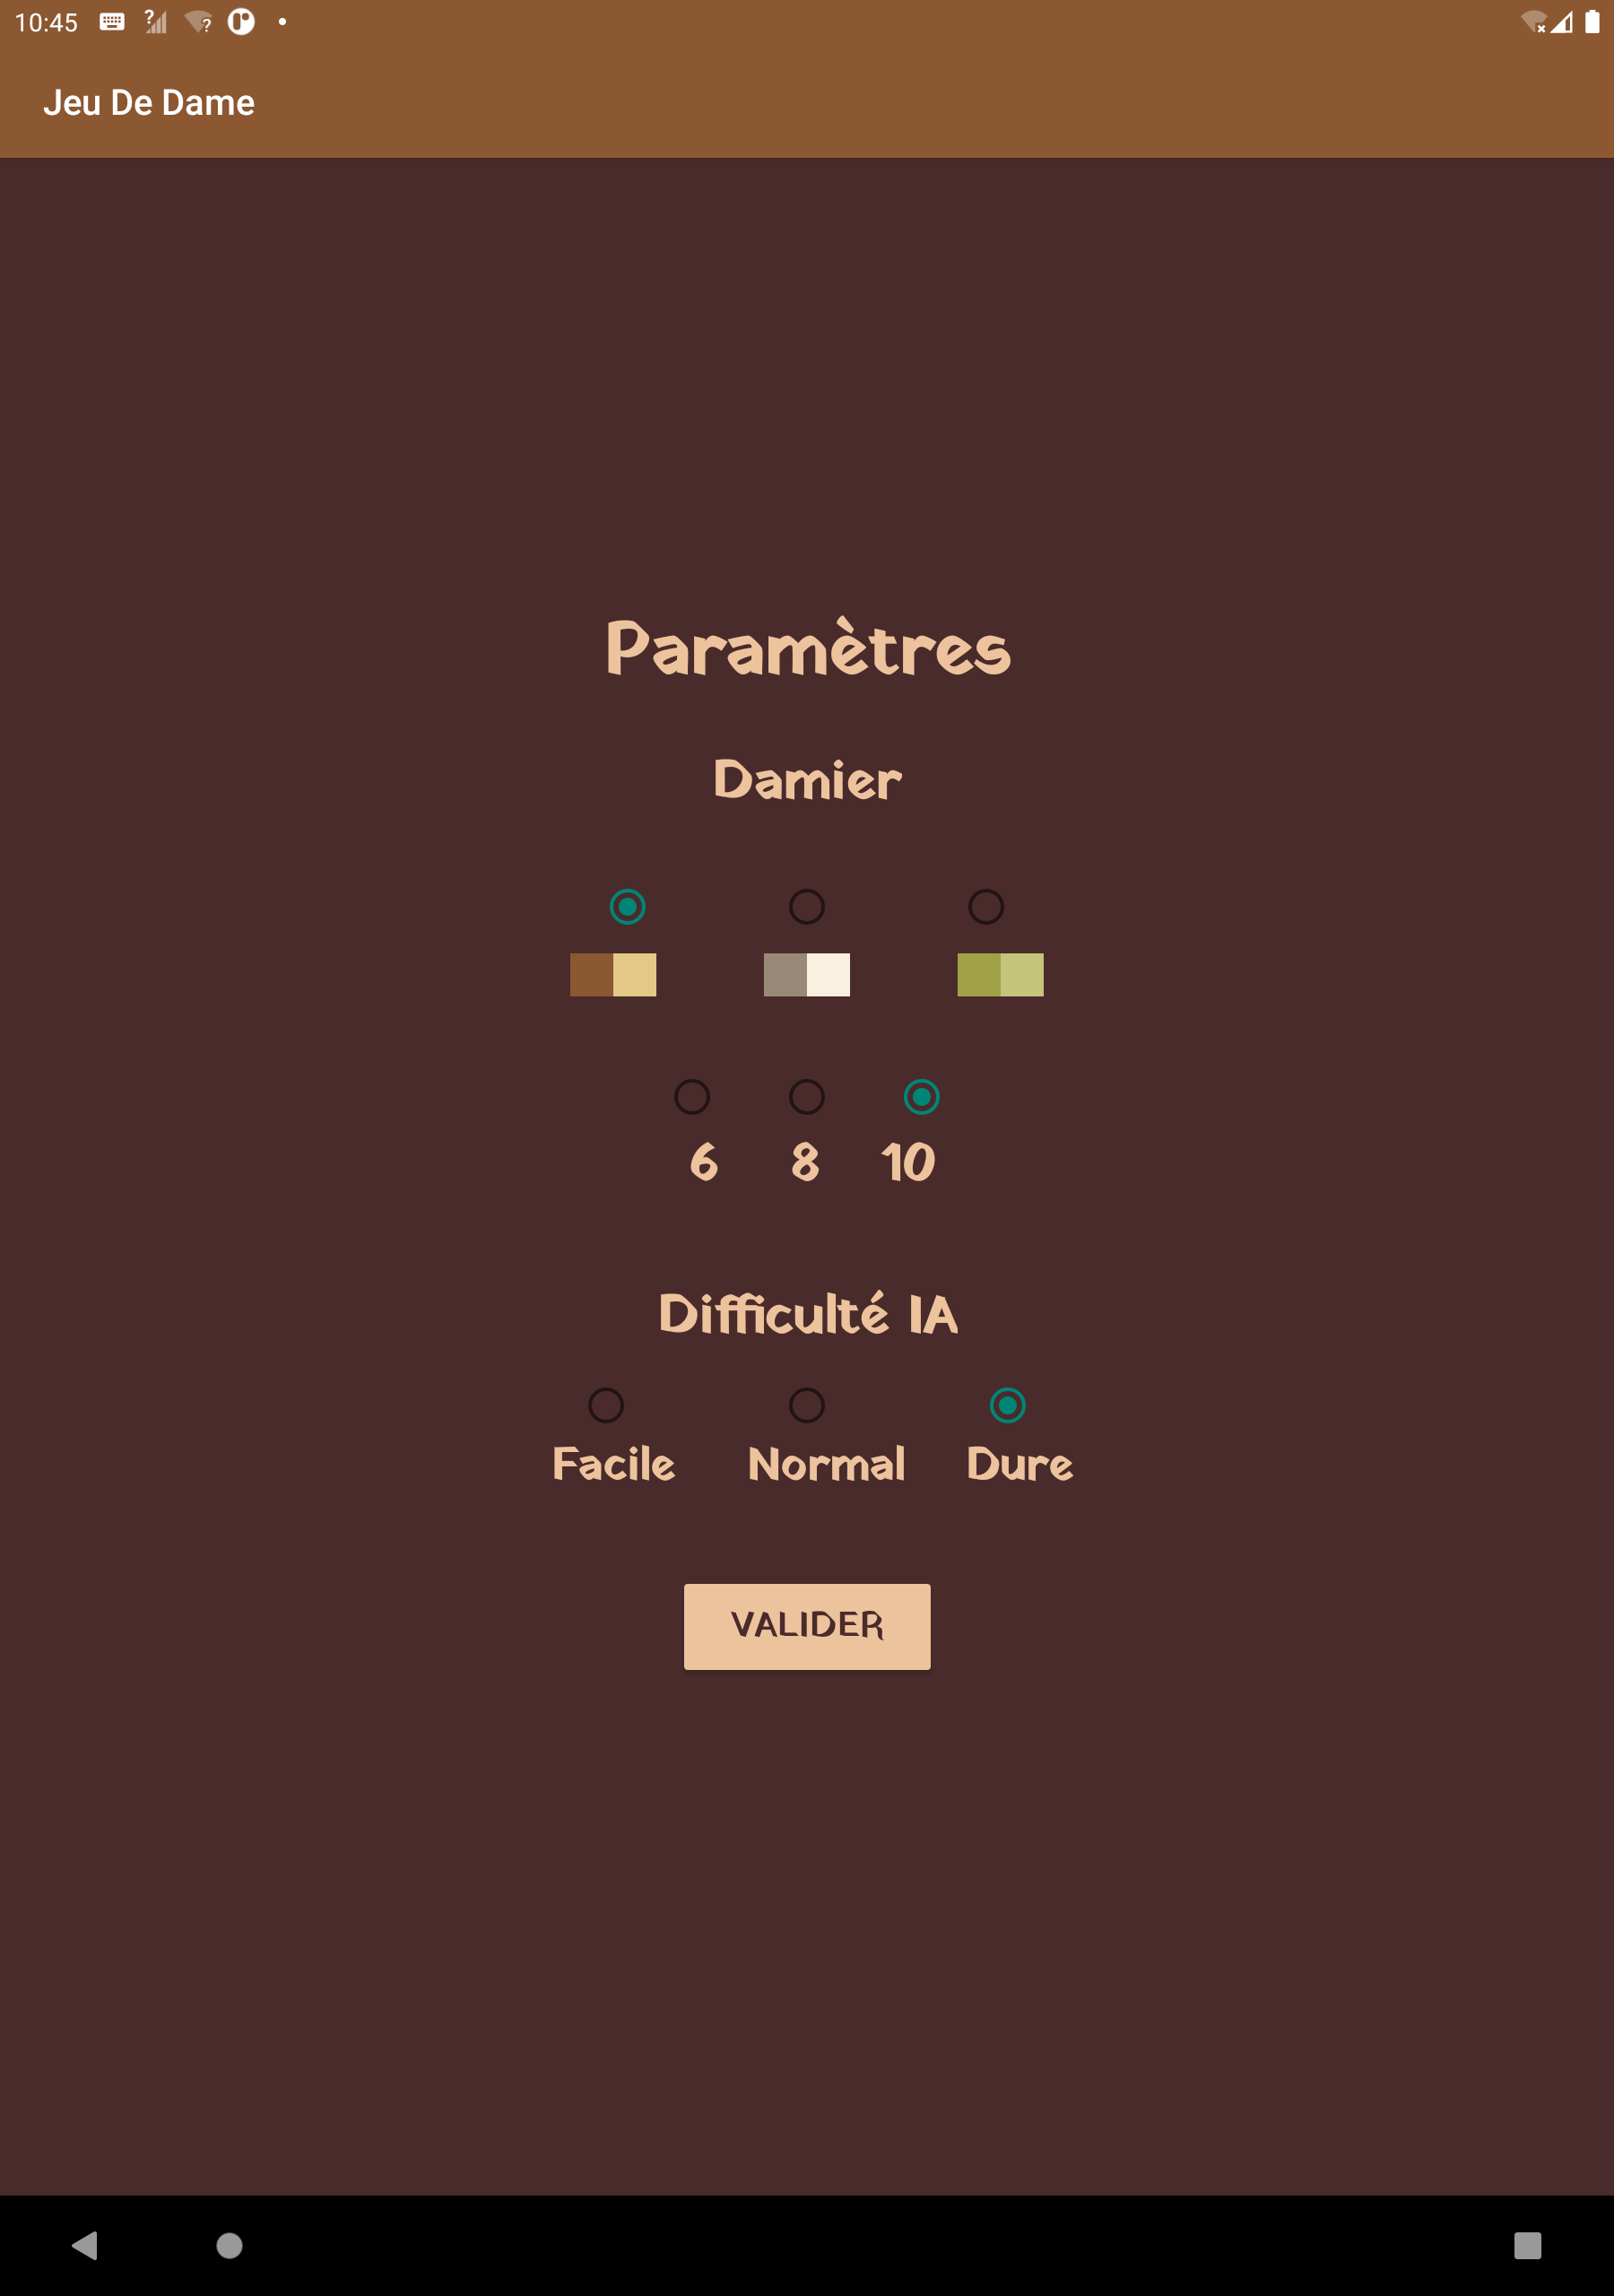
\includegraphics[scale=0.1]{setting_tablet_fr.png}
  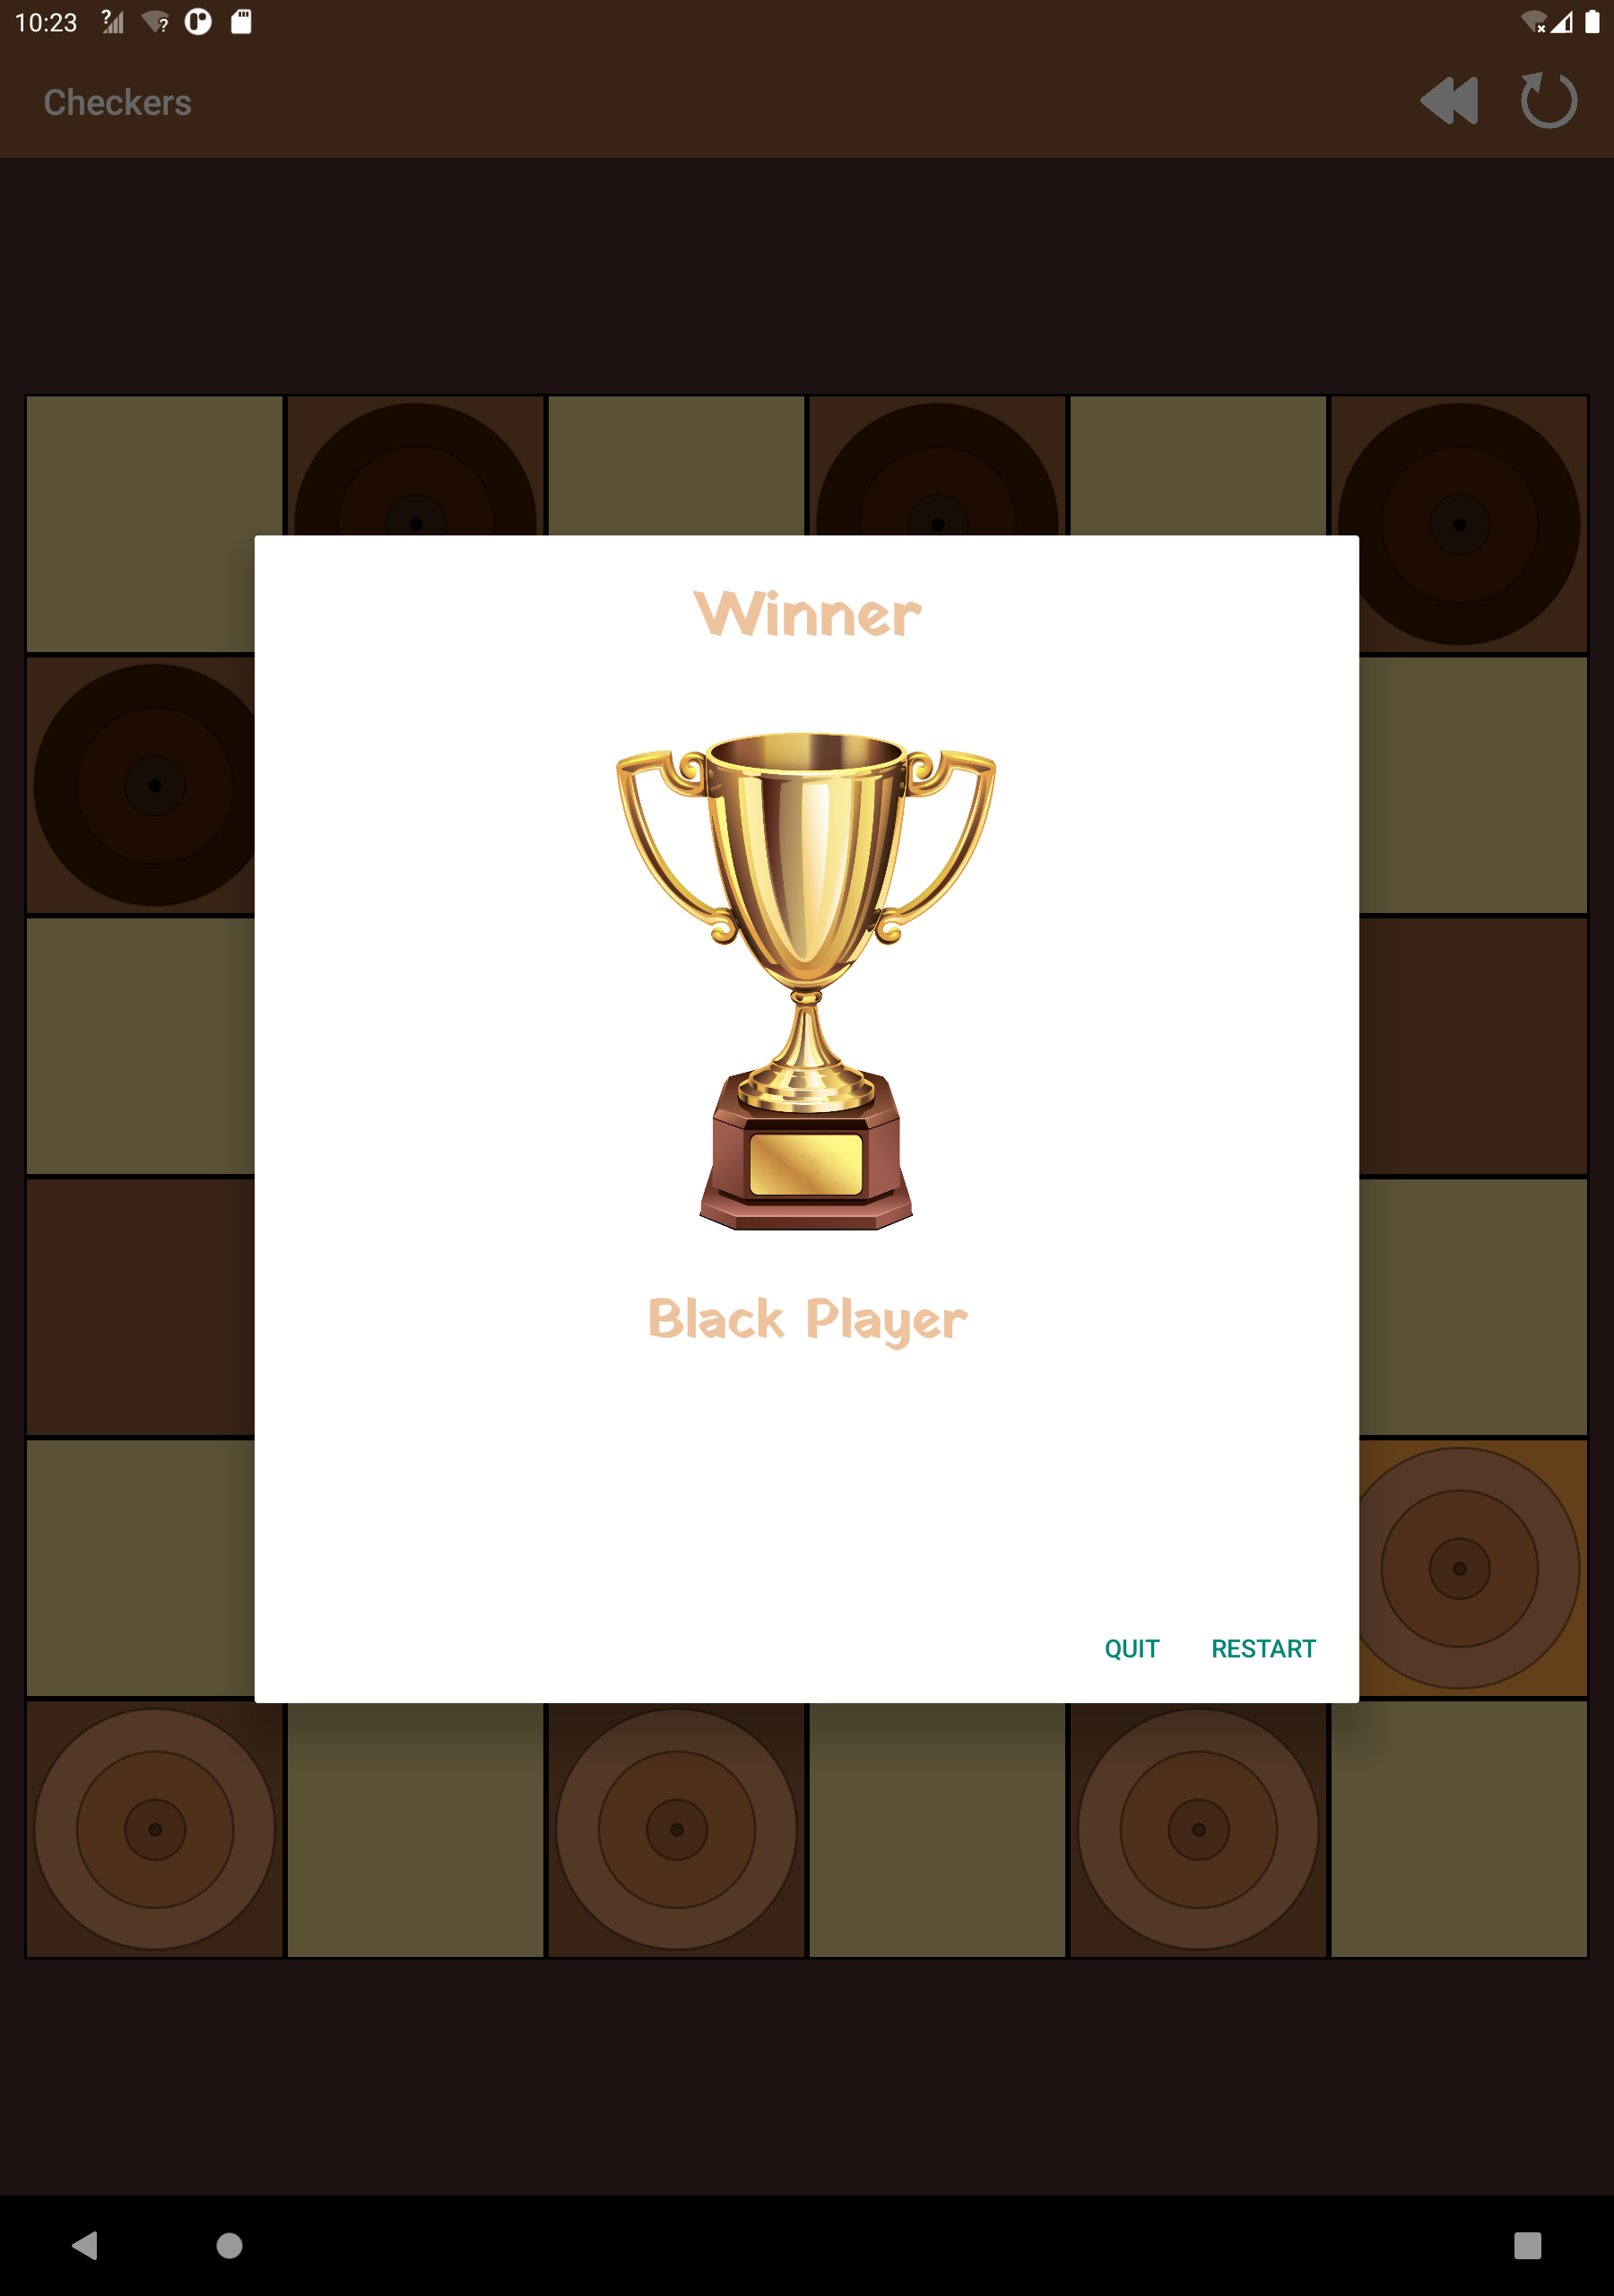
\includegraphics[scale=0.1]{pop_up_victoire_tablet.png}
\end{center}

\end{enumerate}

Et enfin, un petit pop up sympa lorsqu'un joueur gagne la partie, ça n'a pas de prix

\section{Architecture du code}

L'implémentation du jeu est différente sur les deux plateformes.

En éffet, au début du projet du projet, nous étions parti sur une même base.

Mais pour implementer l'IA sur Android, on a du retravaillé tout la struture du code
 (ce qui fut une bonne idée d'ailleurs)

\subsection{Android} %% une sous-section

La structure du code adopté pour l'application sur Android se veut plus précis et éfficace 
mais moins académique. 

En effet, dans l'implémentation, on a éviter de mettre beacoup de classes utilitaires unitiles
comme Joueur, Plateau, Piece, etc... 

\textbf{Voici le diagramme de classe de la version Android: }

\begin{center}
  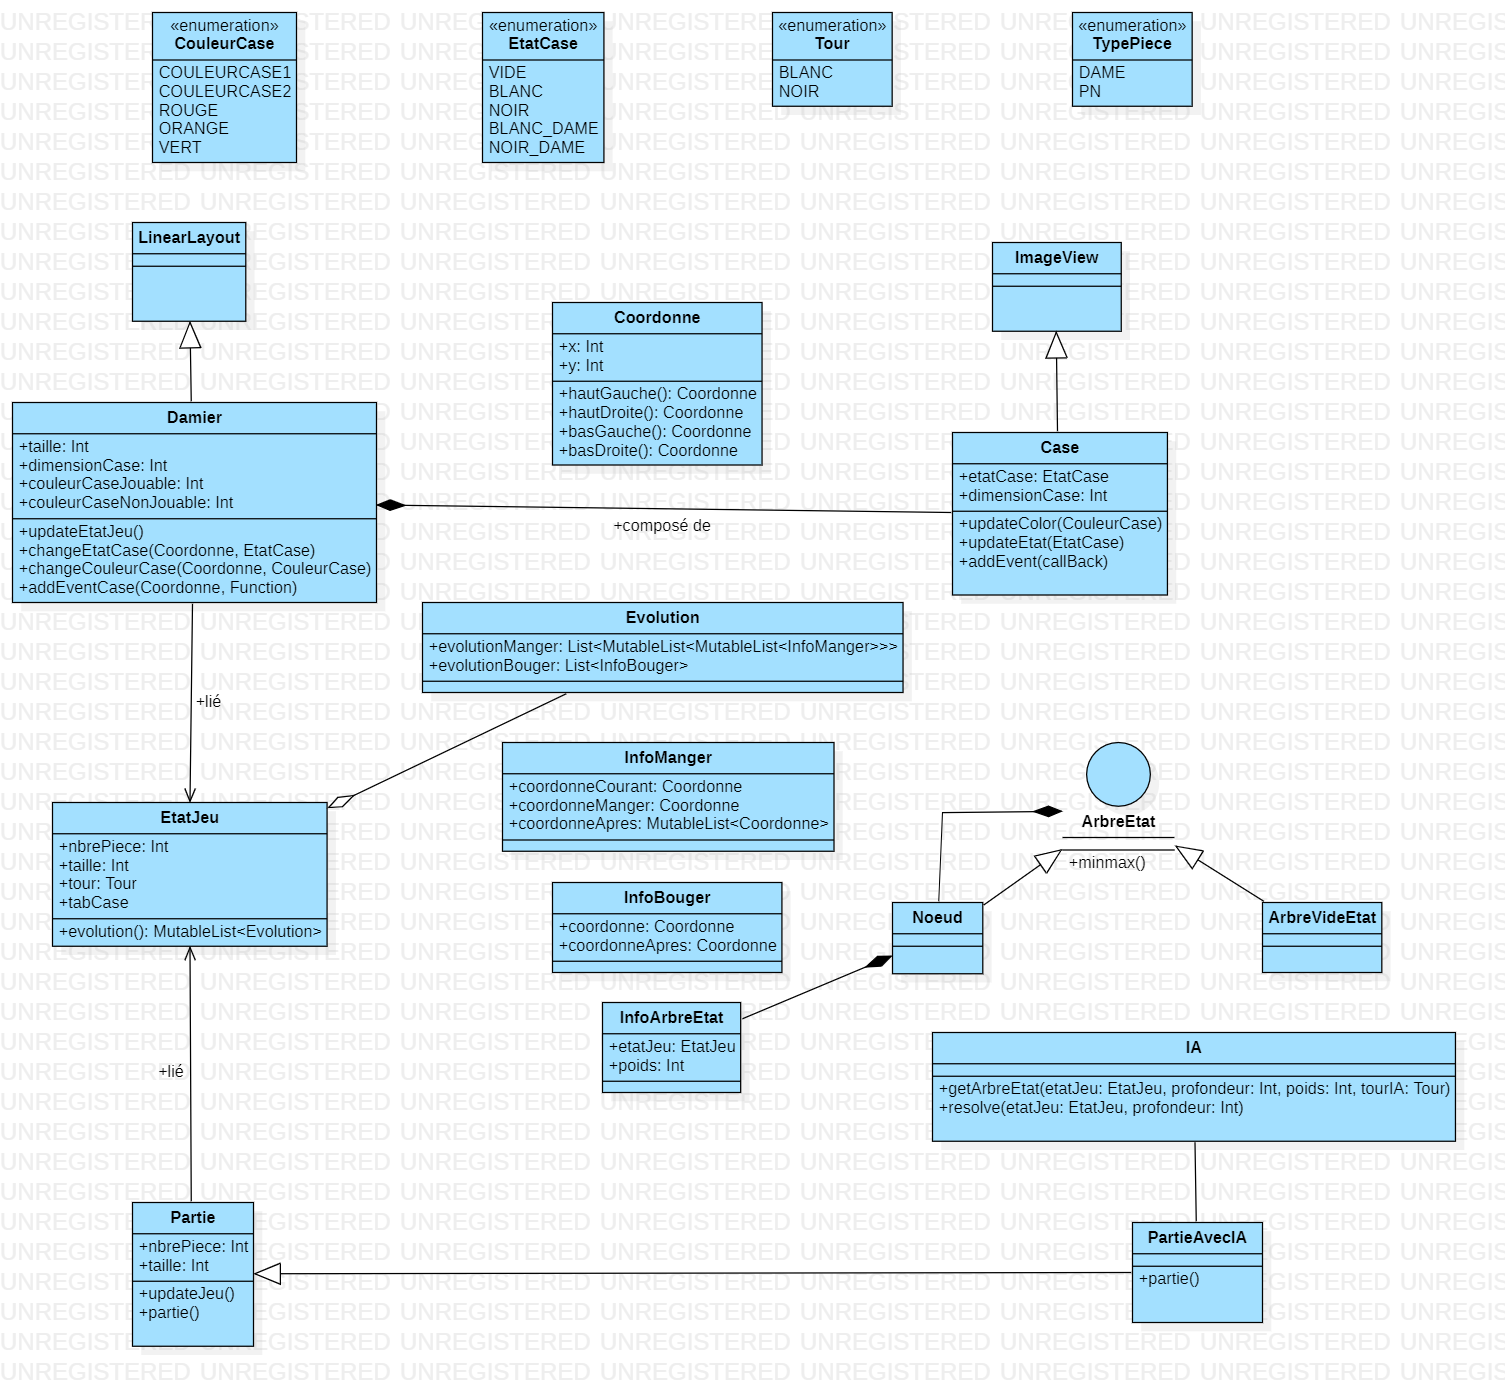
\includegraphics[scale=0.26]{diagramme.png}
\end{center}

En résumé:

  \subsubsection{EtatCase (Model)}

  Cette classe représente l'état du Jeu à un instant donné. 
  Cela se représente très facilement par un \textbf{List<List<EtatCase>>}

  Avec cette classe, on a la possibilité de retourner tout les évolutions possible du jeu.
  C'est à dire, les cases que l'on pourra manger et les endroits où on pourra se déplacer.

  Les méthodes manger et bouger permettent à partir des classes 
  \textbf{InfoManger} et \textbf{InfoBouger} de retourner une nouvelle \textbf{EtatJeu} avec les 
  changements adéquats.

  Cela nous permet de faire évoluer notre partie et de mettre en place un IA
  
  \subsubsection{Damier (Vue)}
  
  Cette classe est un \textbf{LinearLayout} qui va contenir des \textbf{Case} 
  qui sont des \textbf{ImageView}.

  C'est elle qui va afficher le damier et qui va mettre en place tout la partie Vue 
  de notre jeu. 
  C'est elle aussi qui gère les evenements sur les cases.

  \subsubsection{Partie (Controlleur)}
  
  Cette classe permet la liaison entre la vue \textbf{Damier} et le model \textbf{EtatCase}
  et permet de mettre en place les evenement, colorier les cases, etc... 

  \subsubsection{IA}


\textbf{Extrait de code de la fonction minMax}
\begin{verbatim}
  fun minMax(tourIA: Tour): Int {

        return when(this) {

            is ArbreVideEtat -> 0
            is NoeudArbreEtat ->

                if ( fils.all { it is ArbreVideEtat } ) infoArbreEtat.poids
                else {

                    if (infoArbreEtat.etatJeu.tour === tourIA) 
                        max(fils.map { it.minMax(tourIA) } as MutableList<Int>)
                    else min(fils.map { it.minMax(tourIA) } as MutableList<Int>)

                }
            else -> 0
        }

    }
\end{verbatim}

\subsection{iOS} %% une autre sous-section


\section{Quelques points délicats/intéressants}


\section{Conclusion}


%%% La bibliographie:
\bibliographystyle{plain}
\bibliography{ma_biblio}

\end{document}
